\section{Классификация}
\subsection{Общий подход к классификации через апостериорные вероятности} % (fold)
	Общая подход к классификации: строятся классифицирующие функции $f_i$, такие что классификация проводится так:
индивид с признаками $\mathbf{x}$ относится к группе с максимальным значением на нем классифицирующей функции:
$\argmax_i\mathrm f_i(\mathbf{x})$.

 Откуда берутся эти классифицирующие функции? Естественная идея взять в качестве $f_i$ вероятность (ее оценку)
принадлежности к $i$-му классу.
Пусть $\xi$ -- дискретная с.в., принимающая значения $\left\lbrace A_i\right\rbrace_{i=1}^k$, $\mathcal P(\eta\mid \xi = A_i) = \mathcal P_i$ и имеет плотность $p_i(\mathbf{x})$. Тогда было бы логично взять $f_i = p_i$. Для практического применения надо было бы оценить плотности, либо непараметрически (например, по числу точек, попавших в дельта-окрестность --- типа метода ближайших соседей), либо параметрически (если известно, что распределение нормальное, тогда просто оцениваем векторы средних и ковариационные матрицы).

Более сложный подход --- через апостериорные вероятности. Если у нас есть априорное знание вероятности того, что индивид
из того или иного класса, то мы можем его учесть.
Введем понятие класса $C_i = \left\lbrace\xi = A_i\right\rbrace$.  Чтобы классифицировать наблюдение $\mathbf{x}$, необходимо найти
	$$\argmax\mathrm P\left(\xi = A_i\middle\vert \eta = \mathbf{x}\right) = \argmax\mathrm P\left(C_i\middle\vert \mathbf{x}\right).$$

	Пусть известны априорные вероятности принадлежности нового наблюдения к $i$-му классу $\pi_i = \mathrm P\left(C_i\right)$. Тогда апостериорные вероятности по формуле Байеса будут иметь вид $$\mathrm P\left(C_i\middle\vert \mathbf{x}\right) = \frac{\mathrm P\left(\mathbf{x}\middle\vert C_i\right) \pi_i}{\sum_{j=1}^k \mathrm P\left(\mathbf{x}\middle\vert C_j\right) \pi_j}.$$
Поэтому в качестве классифицирующих функций берут
$$f_i\left(\mathbf{x}\right) = \frac{p_i(\mathbf{x}) \pi_i}{\sum_{j=1}^k p_j(\mathbf{x}) \pi_j}. $$

	Так как знаменатель у всех $f_i$ одинаковый, его можно отбросить, и итоговые классифицирующие функции будут выглядеть как $f_i\left(\mathbf{x}\right) = \mathrm P\left(\mathbf{x}\middle\vert C_i\right) \pi_i = p_i(\mathbf{x}) \pi_i$.

	Как выбрать априорные вероятности?

	\begin{enumerate}
		\item Равномерно, $\forall i \in 1\mathbin : k \; \pi_i = 1 \mathbin / k$.
		\item По соотношениям в обучающей выборке: $\pi_i = n_i \mathbin / \sum_{j=1}^k n_j$.
		\item На основе другой дополнительной информации о данных (результаты предыдущих исследований, etc.)
	\end{enumerate}

\begin{prop}
Построенный метод классификации $\mathrm{predict}(\mathbf{x}) = \argmax_i \pi_i p_i(\mathbf{x})$ минимизирует среднюю апостериорную ошибку:
$$\sum_{i=1}^k \pi_i \mathrm P(\mathrm{predict}(\mathbf{x}) != i\mid C_i).$$
\end{prop}

Видно, что можно с помощью априорных вероятностей формально задавать важность ошибочных классификаций
для разных классов.

%\end{document}
\subsection{Линейный и квадратичный дискриминантный анализ для классификации}
	\subsubsection{LDA} % (fold)
	\label{ssub:lda}
		Модель: $\xi$ --- дискретная с.в., принимающая значения $\left\lbrace A_i\right\rbrace_{i=1}^k$, $\mathcal P(\eta\mid \xi = A_i) = \mathcal N\left(\bm{\mu}_i, \bm{\Sigma}\right)$. Тогда плотность в точке $\mathbf{x}$
		$$p_i(\mathbf{x}) = p\left(\mathbf{x}\middle\vert \xi = A_i\right) = \frac{1}{\left(2\pi\right)^{p/2}\left\vert\bm{\Sigma}\right\vert^{1/2}} \exp\left(-\frac{1}{2}\Tr{\left(\mathbf{x} - \bm{\mu}_i\right)}\bm{\Sigma}^{-1}\left(\mathbf{x} - \bm{\mu}_i\right)\right),$$
		и классифицирующая функция $f_i\left(\mathbf{x}\right) = \pi_i p\left(\mathbf{x}\middle\vert \xi = A_i\right)$, где $\pi_i$ --- априорная вероятность наблюдения попасть в $i$-ю группу. Для упрощения вычислений можно переписать классифицирующую функцию через возрастающее монотонное преобразование как

		$$g_i\left(\mathbf{x}\right) = \log f_i\left(\mathbf{x}\right) = \log \pi_i - \frac{1}{2}\log\left\vert\bm{\Sigma}\right\vert -  \frac{1}{2}\Tr{\left(\mathbf{x} - \bm{\mu}_i\right)}\bm{\Sigma}^{-1}\left(\mathbf{x} - \bm{\mu}_i\right).$$
Сократив часть, не зависящую от номера класса, получаем линейные классифицирующие функции
$$h_i(\mathbf{x}) = -\frac{1}{2}\Tr{\bm{\mu}_i}\bm{\Sigma}^{-1}\bm{\mu}_i + \Tr{\bm{\mu}_i}\bm{\Sigma}^{-1}\mathbf{x} + \log\pi_i.$$

\begin{note}
  Если две группы, то гипотеза о равенстве многомерных мат.ож. $H_0: \bm{\mu}_1 = \bm{\mu}_2$ (различие значимо, если гипотеза отвергается, а только тогда имеет смысл проводить классификацию) в модели LDA проверяется с помощью критерия Хотеллинга (Hotelling). Если групп несколько, то есть разные критерии, например, критерия Wilk's Lambda или Roy's greatest root (эти же критерии используются в MANOVA, Multivariate ANalysis Of VAriance). Они отличаются мощностью против разного расположения групп.
\end{note}

\paragraph{Проверка гипотезы о равенстве двух многомерных мат. ожиданий, независимые выборки (two-sample)}
Пусть $\bm\xi^{(1)},\bm\xi^{(2)} \in \R^p$  --- независимые. При этом первая выборка имеет размер $n_1$, а вторая --- $n_2$. Проверяем гипотезу:

$H_0: \mathbb{E}\bm\xi^{(1)} = \mathbb{E}\bm\xi^{(2)}$ ($H_0: \bm\mu_1 = \bm\mu_2$).

Пример: есть 2 группы людей. Снимаются показания по росту, весу, длине рук и т.д. Необходимо сравнить ``средние размеры''. Рассмотрим случаи:
\begin{itemize}
\item $\bf\Sigma_1 = \bf\Sigma_2 = \bf\Sigma$ --- известна. Тогда статистика критерия имеет вид:
%
\begin{equation*}
t = (\bar{\mathbf{x}}^{(1)} - \bar{\mathbf{x}}^{(2)})^{\mathrm{T}} \Big (\bm\Sigma (\frac{1}{n_1} + \frac{1}{n_2}) \Big )^{-1} (\bar{\mathbf{x}}^{(1)} - \bar{\mathbf{x}}^{(2)}) \sim \chi^2 (p),
\end{equation*}
%
где $\bm\xi^{(i)} \sim \mathcal{N}_p (\bm\mu_i,\bm\Sigma)$ (иначе, $\chi^2 (p)$ асимптотически). Статистика критерия --- расстояние Махаланобиса от $(\bar{\mathbf{x}}^{(1)} - \bar{\mathbf{x}}^{(2)})$ до 0, $\bm\Sigma (\frac{1}{n_1} + \frac{1}{n_2})$ --- ковариационная матрица разности (но тут ковариационная матрица одинаковая для обеих выборок, поэтому в формуле такое выражение). Вообще говоря, $\cov \bar{\mathbf{x}} = \cov \bm\xi/n$.

\item $\bm\Sigma_1 = \bm\Sigma_2 = \bm\Sigma$ --- неизвестна. Тогда берем pooled covariance matrix $\tilde{\mathbf{S}} = \frac{(n_1 - 1)\tilde{\mathbf{S}}^{(1)} + (n_2 - 1)\tilde{\mathbf{S}}^{(2)}}{n_1 + n_2 - 2}$, где $\tilde{\mathbf{S}}^{(1)}, \tilde{\mathbf{S}}^{(2)}$ --- исправленные выборочные ковариационные матрицы для векторов $\bm\xi^{(1)}, \bm\xi^{(2)}$, соответственно.
Статистика критерия:
%
\begin{equation*}
t = (\bar{\mathbf{x}}^{(1)} - \bar{\mathbf{x}}^{(2)})^{\mathrm{T}} \Big (\tilde{\mathbf{S}} (\frac{1}{n_1} +
\frac{1}{n_2}) \Big )^{-1} (\bar{\mathbf{x}}^{(1)} - \bar{\mathbf{x}}^{(2)}) \sim T_p^2 (n_1+n_2-2),
\end{equation*}
%
где $\bm\xi^{(i)} \sim \mathcal{N}_p (\bm\mu,\bm\Sigma)$ (иначе, асимптотически). Здесь $T_p$ обозначено так называемое распределение Хотеллинга (Hotelling).

\item Неизвестно, что $\bm\Sigma_1 = \bm\Sigma_2$. 
Статистика критерия:
%
\begin{equation*}
t = (\bar{\mathbf{x}}^{(1)} - \bar{\mathbf{x}}^{(2)})^{\mathrm{T}} \Big (\frac{\tilde{\mathbf{S}}_1}{n_1} +
\frac{\tilde{\mathbf{S}}_2}{n_2} \Big )^{-1} (\bar{\mathbf{x}}^{(1)} - \bar{\mathbf{x}}^{(2)}) \xrightarrow[n_1, n_2
\rightarrow \infty]{\sim} \chi^2 (p).
\end{equation*}
%
\end{itemize}

\paragraph{Проверка гипотезы о равенстве ковариационных матриц}
Пусть $\bm\xi^{(i)} \in \R^{p}, \bm\xi^{(i)} \sim \mathcal{N}_p (\bm\mu_i, \bm\Sigma_i), i = 1, \dots, k$. Проверяем гипотезу (о гомоскедастичности):
$H_0: \bm\Sigma_1 = \dots = \bm\Sigma_k$.
 Считаем несмещенные оценки ковариационных матриц $\tilde{\mathbf{S}}_i$, определим
%
\begin{equation*}
M = \Big (\frac{|\tilde{\mathbf{S}}_1|}{|\tilde{\mathbf{S}}|} \Big )^{\nu_1/2} \dots  \Big (\frac{|\tilde{\mathbf{S}}_k|}{|\tilde{\mathbf{S}}|} \Big )^{\nu_k/2},
\end{equation*}
%
где $\nu_i = n_i - 1$ --- число степеней свободны, а $\tilde{\mathbf{S}} = \frac{(n_1 - 1)\tilde{\mathbf{S}}_1 + \cdots + (n_k - 1)\tilde{\mathbf{S}}_k}{n_1 + \cdots + n_k - k}$ --- pooled covariance matrix.

Считаем статистику критерия (\underline{Box's statistics}), ее распределение известно:
%
\begin{equation*}
t = - \log M
\end{equation*}
%

При отклонении от нормальности критерий становится неправильным.

\paragraph{Значимость LDA. MANOVA}
%не надо в заголовках математику, она с hypperlink плохо
%работает
Общая постановка задачи.
Пусть есть $k$ групп и $p$ признаков, мы хотим проверить гипотезу, что группы друг от друга не отличаются. Если гипотеза отвергается, то отличие значимо.

Формально есть $k$ (многомерных) случайных векторов $\bm \eta_1, \ldots, \bm \eta_k \in \R^p$ и гипотеза формулируется так:

\begin{equation}
    \label{PreMANOVA}
    \mathrm H_0: \mathcal P(\bm \eta_1) = \mathcal P(\bm \eta_2) = \ldots = \mathcal P(\bm \eta_k).
\end{equation}
Эту задачу можно переформулировать следующим образом.
Пусть есть дискретный (м.б. качественный) признак $\xi$, принимающий ровно $k$ значений: $A_1, A_2, \ldots, A_k$.
Рассмотрим случайный вектор $\Tr{(\bm \eta, \xi)} \in \R^k \times \{A_1, A_2, \ldots, A_k\}$,
такой что $\mathcal P(\bm \eta \, | \, \xi = A_i) = \mathcal P(\eta_i)$ для всех $i \in 1:k$.
Тогда гипотеза \eqref{PreMANOVA} переписывается в виде:
\begin{equation}
    \label{PreMANOVA2}
    \mathrm H_0^*: \mathcal P(\bm \eta \, | \, \xi = A_1) = \ldots = \mathcal P(\bm \eta \, | \, \xi = A_k).
\end{equation}

В MANOVA рассматривается частный случай (модель), когда $\mathcal P(\bm \eta_i) = \mathcal N(\bm \mu_i, \Sigma)$.
В рамках этой модели гипотезам \eqref{PreMANOVA} и \eqref{PreMANOVA2} равносильны следующие две равносильные гипотезы:
\begin{gather}
    \label{MANOVA}
    \mathrm H_0: \bm \mu_1 = \bm \mu_2 = \ldots = \bm \mu_k.\\
    \mathrm H_0^*: \mathbb E (\bm \eta \, | \, \xi = A_1) = \ldots = \mathbb E (\bm \eta \, | \, \xi = A_k).
    \nonumber
\end{gather}

Многомерное Основное Дисперсионное Тождество можно записать на генеральном языке как
\begin{gather}
    \label{MANOVA_VI_gen}
    \mathrm {Cov} \bm \eta =
    \mathbb E \big[(\bm \eta - \mathbb E \bm \eta) \Tr{(\bm \eta - \mathbb E \bm \eta)}\big] = \\ =
    \mathbb E \big[(\bm \eta - \mathbb E (\bm \eta \, | \, \xi))
              \Tr{(\bm \eta - \mathbb E (\bm \eta \, | \, \xi))}\big] +
    \mathbb E \big[(\mathbb E (\bm \eta \, | \, \xi) - \mathbb E \bm \eta)
              \Tr{(\mathbb E (\bm \eta \, | \, \xi) - \mathbb E \bm \eta)}\big].
\end{gather}

Поэтому гипотеза MANOVA формулируется так: 
\begin{gather}
    \label{MANOVA_VI_H}
    \mathrm H_0:
    \mathbb E \big[(\mathbb E (\bm \eta \, | \, \xi) - \mathbb E \bm \eta)
              \Tr{(\mathbb E (\bm \eta \, | \, \xi) - \mathbb E \bm \eta)}\big]
    = 0.
\end{gather}
Эта запись является многомерным обобщением ANOVA и так же означает, что средние внутри групп не отличаются от общего среднего.

Выборка задается так же как в ANOVA, но теперь индивиды многомерные.
Имеется $n_i$ индивидов из $i$-той группы ($i \in 1:k$).
Обозначим $\mathbf y_{ij} \in \R^p$%\footnote{\color{blue} Шрифт тут неудачный, но пусть пока так будет}
--- $j$-того индивида из $i$-той группы ($i \in 1:k$ и $j \in 1:n_i$).
Обозначим $\overline {\mathbf y}$ --- выборочное среднее по всем индивидам, а $\overline {\mathbf y_i}$
--- выборочное среднее индивидов $i$-той группы.

Запишем \eqref{MANOVA_VI_gen} на выборочном языке:
\begin{gather}
    \label{VI_MANOVA}
    \sum_{i=1}^k \sum_{j=1}^{n_i} (\mathbf y_{ij} - \overline {\mathbf y}) \Tr{(\mathbf y_{ij} - \overline {\mathbf y})} =
    \sum_{i=1}^k n_i (\overline {\mathbf y_i} - \overline {\mathbf y}) \Tr{(\overline {\mathbf y_i} - \overline {\mathbf y})} +
    \sum_{i=1}^k \sum_{j=1}^{n_i} (\mathbf y_{ij} - \overline {\mathbf y_i}) \Tr{(\mathbf y_{ij} - \overline {\mathbf y_i})}.
\end{gather}

Первое слагаемое отвечает за равенство средних (неотличимые группы), его назовем $\mathbf{H}$ от слов hypothesis, а второе --- за отклонение данных в каждой группе от своего среднего, его назовем $\mathbf{E}$ от слова error:
\begin{gather*}
    \mathrm {\mathbf E} \overset{\mathrm{def}}{=}
    n\widehat {\mathbb E \big[(\bm \eta - \mathbb E (\bm \eta \, | \, \xi))
    \Tr{(\bm \eta - \mathbb E (\bm \eta \, | \, \xi))}\big]} =
    \sum_{i=1}^k \sum_{j=1}^{n_i} (\mathbf y_{ij} - \bm {\mathbf y_i}) \Tr{(\mathbf y_{ij} - \bm {\mathbf y_i})};\\
    \mathrm {\mathbf H} \overset{\mathrm{def}}{=}
    n\widehat{\mathbb E \big[(\mathbb E (\bm \eta \, | \, \xi) - \mathbb E \bm \eta)
    \Tr{(\mathbb E (\bm \eta \, | \, \xi) - \mathbb E \bm \eta)}\big]} =
    \sum_{i=1}^k n_i (\bm {\mathbf y_i} - \bm {\mathbf y}) \Tr{(\bm {\mathbf y_i} - \bm {\mathbf y})}.
\end{gather*}


Стоит сразу отметить, что, когда в дальнейшем мы будем строить критерии для проверки значимости,
мы всегда будем их строить, как некие преобразования над парой матриц $(\mathbf H, \mathbf E)$.

Пусть $\lambda_i$  --- упорядоченные по убыванию собственные числа матрицы $\mathbf{E}^{-1}\mathbf{H}$ (можно доказать, что они неотрицательные, так как $\mathbf{E}$ --- симметричная неотрицательно определенная матрица).
Число ненулевых собственных чисел равно $s\le \min(n, k-1)$.

\paragraph{Смысл $\lambda_i$. Канонические переменные}

В LDA есть так называемые канонические переменные. Идея похожа на АГК, только оптимизационная задача другая. Аналогично, на основе исходных признаков (признаки центрируются) строятся новые признаки как линейные комбинации исходных признаков. Только первая каноническая переменная --- это такая линейная комбинация исходных признаков, по которой группа максимально отличаются (отличие измеряется на основе ANOVA, по статистике критерия Фишера, с точностью до коэффициента это $\lambda_1$). Вторая линейная комбинация должна быть ортогональна первой и приводит к максимальному различию среди ортогональных линейных комбинаций (мера отличия $\lambda_2$). И т.д. Удобно смотреть на данные в плоскости первой и второй канонических переменных (иногда это называют roots).

Формализуем.

Запишем на генеральном языке, что значит <<новый признак>>. Есть $A \in \R^p$ и новый признак
$\zeta = \Tr{A} \bm\eta$: $\mathcal P(\zeta \, | \, \xi = A_i) = \mathcal N(\Tr{A} \bm\mu_i, \Tr{A} \bm\Sigma A)$.
На выборочном языке --- $Z = \mathbf Y A$ и выборочная ковариационная матрица (с точностью до коэффициента имеет вид):
$\Tr{A} \Tr{\mathbf Y} \mathbf Y A = \Tr{A} ( \mathbf H + \mathbf E ) A$. Из этого следует, %\footnote{\color{blue} Кто-то умеет формально
%это доказывать? Это нужно делать как-то на генеральном языке видимо, пользуясь ортогональностью.},
что <<аналогом>> $\mathbf H$ для
нового признака является $\Tr{A} \mathbf H A$, а аналогом $\mathbf E$ является $\Tr{A} \mathbf E A$.
%\footnote{Чтобы в этом убедиться, нужно написать оценкой чего является $\mathbb H$ и $\mathbb E$. Дальше домножить это на $A$ нужным образом
%и ввести обозначение для нового признака. Дальше все станет ясно.}

Посмотрим теперь на $F$-статистику для ANOVA:

\begin{gather*}
    F = F(A) = C \frac{\mathrm{SSH}_\zeta}{\mathrm{SSE_\zeta}} = C \frac{\Tr{A} \mathbf H A}{\Tr{A} \mathbf E A} \sim
    \mathrm F_{\nu_\mathbf H, \nu_\mathbf E}.
\end{gather*}
где $C = \nu_\mathbf E / \nu_\mathbf H$ --- коэффициент, не зависящий от $A$.

Исходно ставилась задача --- найти такие признаки, по которым группы <<наиболее бы отличались>>, причем желательно, чтобы признаки были ортогональны.
В терминах статистики $F$ в ANOVA --- это означает, %\footnote{Приглашаю убедиться.} 
Таким образом, решается обобщенная задача на собственные числа и собственные вектора (в обычной задаче матрица $\mathbf E$ единичная:
\begin{gather*}
    \frac{\Tr{A} \mathbf H A}{\Tr{A} \mathbf E A} \rightarrow \max_A.
\end{gather*}

Собственные числа матрицы $\mathbf E^{-1} \mathbf H$ в порядке невозрастания: $\lambda_1 \geqslant \lambda_2 \geqslant \ldots
\geqslant \lambda_s$, где $s = \min\{p, \nu_H\}$, и собственные вектора той же матрицы $A_i$ для $i \in 1:s$.
Причем $\Tr{A_i} \mathbf E A_j = 0$ для $j < i$.
Вектора $A_i$ --- канонические коэффициенты (дискриминантные функции). Новые признаки $Z_i = \mathbf Y A_i$ --- канонические переменные.
Можно формально доказать, что новые признаки являются ортогональными.

Исходя из описания, смысл $\lambda_i$ --- степень разброса по $i$-тому направлению, задаваемым $i$-той дискриминантной функцией.
$A_i$ --- коэффициенты с которыми нужно взять исходные признаки, чтобы получить новый признак, имеющий наибольший разброс и ортогональный
предыдущим. А сами канонические переменные тем самым --- ортогональные новые признаки, имеющие наибольший разброс, измеряемый $\lambda_i$.




%Приведем формулу, как находятся коэффициенты линейной комбинации (канонические коэффициенты) для получения канонических переменных. Неудивительно, что экстремальная задача приводит к поиску собственных векторов некоторой матрицы.

%В этих обозначениях, канонические коэффициенты являются собственными векторами матрицы $\mathbf{E}^{-1}\mathbf{H}$. А собственные числа $\lambda_i$ (упорядоченные по убыванию вместе с собственными векторами) этой матрицы отражают то, насколько группы хорошо разделяются по соответствующей канонической переменной. Число ненулевых собственных чисел $s\le \min(n, k-1)$.


\paragraph{Критерии для MANOVA}

Критерии $H_0:\bm\mu_1=\ldots=\bm\mu_k$ являются комбинацией этих собственных чисел. Например:

Статистика критерия Wilks' Lambda $$\Lambda = \prod_{i=1}^s {\frac{1}{1 + \lambda_i}}$$ (с какой стороны критическая область?). 

Статистика критерия Roy's greatest root имеет вид $$r_1^2 = \frac{\lambda_1}{1+\lambda_1} $$ (с какой стороны критическая область?).

Как понять, против какого расположения группы мощнее один, а против какого --- другой?


	\subsubsection{QDA} % (fold)
	\label{ssub:qda}

	Модель: $\xi$ --- дискретная с.в., принимающая значения $\left\lbrace A_i\right\rbrace_{i=1}^k$, $\mathcal P(\eta\mid \xi = A_i) = \mathcal N\left(\bm{\mu}_i, \bm{\Sigma}_i\right)$. Тогда плотность в точке $\mathbf{x}$
		$$p\left(\mathbf{x}\middle\vert \xi = A_i\right) = \frac{1}{\left(2\pi\right)^{p/2}\left\vert\bm{\Sigma}_i\right\vert^{1/2}} \exp\left(-\frac{1}{2}\Tr{\left(\mathbf{x} - \bm{\mu}_i\right)}\bm{\Sigma}_i^{-1}\left(\mathbf{x} - \bm{\mu}_i\right)\right),$$
		и классифицирующая функция $f_i\left(\mathbf{x}\right) = \pi_i p\left(\mathbf{x}\middle\vert \xi = A_i\right)$. Применяем возрастающее монотонное преобразование и оставляем в классифицирующей функции только члены, отличающиеся в разных группах:

		$$g_i\left(\mathbf{x}\right) = \log f_i\left(\mathbf{x}\right) = \log \pi_i - \frac{1}{2}\log\left\vert\bm{\Sigma}_i\right\vert -  \frac{1}{2}\Tr{\left(\mathbf{x} - \bm{\mu}_i\right)}\bm{\Sigma}_i^{-1}\left(\mathbf{x} - \bm{\mu}_i\right),$$
получаем квадратично зависящую от $\mathbf{x}$ классифицирующую функцию.

\begin{note}
  Если две группы, то гипотеза о равенстве многомерных мат.ож. $H_0: \bm{\mu}_1 = \bm{\mu}_2$ (различие значимо, если гипотеза отвергается, а только тогда имеет смысл проводить классификацию) в модели QDA тоже проверяется с помощью критерия Хотеллинга (Hotelling), но с отдельно оцененными ковариационными матрицами (критерий асимптотический). Если групп несколько, то тут уже критерий сложно построить.
\end{note}

%\newpage
\subsection{Классификация в случае двух классов}
Если всего два класса, то можно построить границу между классами, приравняв классифицирующие функции.
\subsubsection{LDA} % (fold)
Приравняв $h_1(x)= h_2(x)$, получим разделяющую гиперплоскость.
Разделяющая два класса гиперплоскость имеет вид
\begin{multline*}
  \{\mathbf{x} : h_1(\mathbf{x}) = h_2(\mathbf{x})\} =\\ = \{\mathbf{x} : -\frac{1}{2} (\bm{\mu}_1 - \bm{\mu}_2)^\mathrm{T} \mathbf{\bm{\Sigma}}^{-1}(\bm{\mu}_1 + \bm{\mu}_2) + (\bm{\mu}_1 - \bm{\mu}_2)^\mathrm{T} \mathbf{\bm{\Sigma}}^{-1}\mathbf{x} + \log(\pi_1/\pi_2) = 0\}.
\end{multline*}
От соотношения между априорными вероятностями зависит положение границы относительно классов (к какому она ближе).
Видно, что априорные вероятности влияют только на сдвиг разделяющей гиперплоскости.

Заметим, что классификацию можно записать как сравнение $-\frac{1}{2} (\bm{\mu}_1 - \bm{\mu}_2)^\mathrm{T} \mathbf{\bm{\Sigma}}^{-1}(\bm{\mu}_1 + \bm{\mu}_2) + (\bm{\mu}_1 - \bm{\mu}_2)^\mathrm{T} \mathbf{\bm{\Sigma}}^{-1}\mathbf{x}$ с некоторым порогом ($-\log(\pi_1/\pi_2)$), который зависит от априорных вероятностей
(или весов ошибок для разных классов, смотря как на это смотреть).

\subsubsection{QDA} % (fold)
	В данном случае, разделяющая поверхность имеет вид квадратичной поверхности, может состоять из двух гиперболоидом,
может иметь форму эллипса.

\subsubsection{Картинки}

	\begin{figure}[!h]
		%\subfigure{
			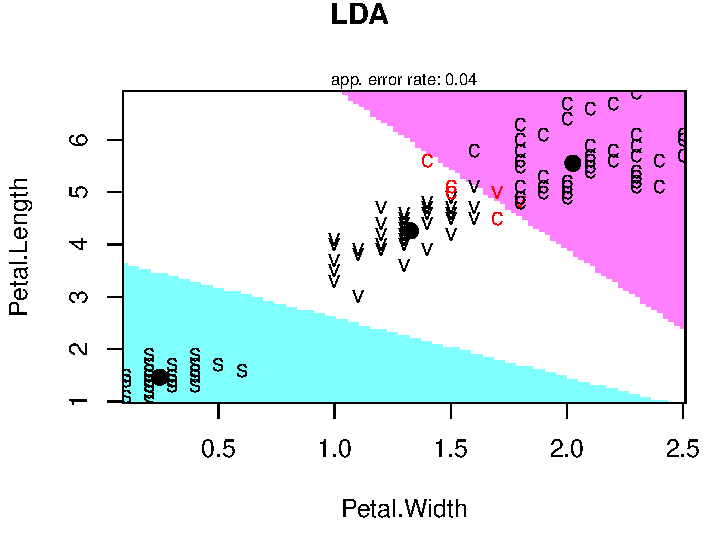
\includegraphics[width=0.5\textwidth]{img/lda.pdf}
			\includegraphics[width=0.5\textwidth]{img/qda.pdf}\\
			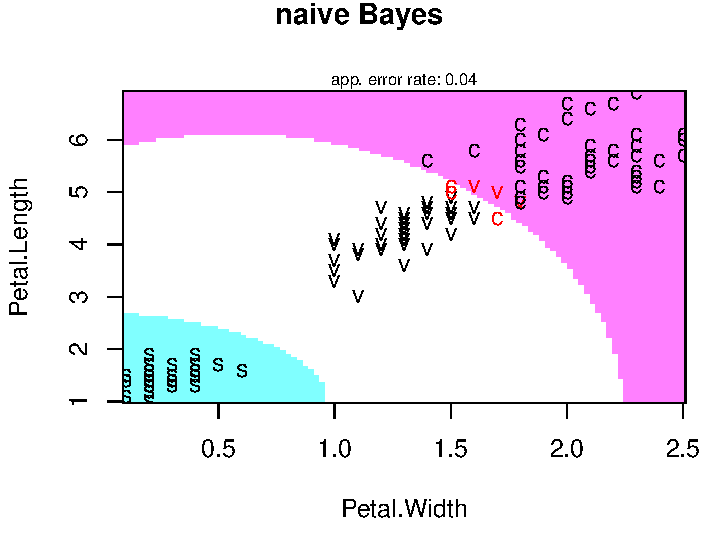
\includegraphics[width=0.5\textwidth]{img/nbda.pdf}
			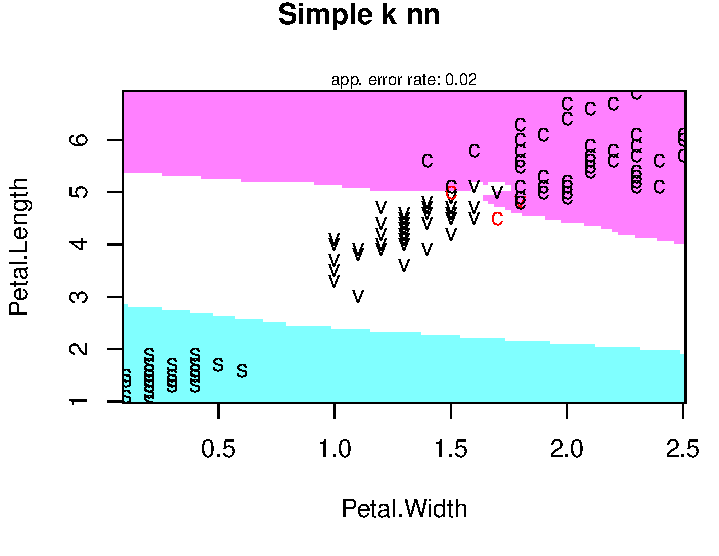
\includegraphics[width=0.5\textwidth]{img/sknn.pdf}
		%}
	\end{figure}

Здесь мы обсуждали число параметров в моделях, возможный overfitting (переподгонку).
Использовали слова --- обобщающая способность алгоритма.

\subsection{Качество классификации}


\subsubsection{Ошибки класификации}

Качество классификации измеряется ошибками классификации (доля неправильно классифицированных объектов).
$n_{ij}$ --- число объектов из класса $i$, отнесенных к классу $j$. В соответствующей матрице классификации
на диагонали стоят правильно классифицированные объекты, вне диагонали --- ошибки.

На самом деле, нельзя проверять качество предсказания на тех данных, на которых это предсказание строилось.
Поэтому используют кросс-валидацию (скользящий контроль).
Например, каждое наблюдение по очереди исключается из выборки, классифицирующее правило строится без него и с
 помощью этого правила индивид классифицируется. Строится аналогичная таблица из $n_{ij}$. В ней ошибок будет,
 вообще говоря, больше.

 Здесь обсуждали, что имеет смысл смотреть на ошибки без кросс-валидации и с ней. Если разница существенная, то
 это говорит о переподгонке используемой модели. Вероятно, она не очень хорошая; например, слишком много
 параметров.

Замечание. Нельзя путать классификацию и различие групп. Группы могут значимо различаться, классификация может
быть при этом бессмысленной
(ошибок чуть меньше 50\%).

\subsubsection{ROC и AUC}

\paragraph{wikipedia}

ROC-кривая (англ. receiver operating characteristic, рабочая характеристика приёмника) --- график, позволяющий оценить качество бинарной классификации, отображает соотношение между долей объектов от общего количества носителей признака, верно классифицированных как несущих признак, (англ. true positive rate, TPR, называемой чувствительностью алгоритма классификации) и долей объектов от общего количества объектов, не несущих признака, ошибочно классифицированных как несущих признак (англ. false positive rate, FPR, величина 1-FPR называется специфичностью алгоритма классификации) при варьировании порога решающего правила.

Также известна как кривая ошибок. Анализ классификаций с применением ROC-кривых называется ROC-анализом.

Количественную интерпретацию ROC даёт показатель AUC (англ. area under ROC curve, площадь под ROC-кривой) — площадь, ограниченная ROC-кривой и осью доли ложных положительных классификаций. Чем выше показатель AUC, тем качественнее классификатор, при этом значение 0,5 демонстрирует непригодность выбранного метода классификации (соответствует случайному гаданию). Значение менее 0,5 говорит, что классификатор действует с точностью до наоборот: если положительные назвать отрицательными и наоборот, классификатор будет работать лучше.

\paragraph{мои комментарии}

Если кто-то хорошо представляет себе, как выглядит график зависимости мощности от ошибки первого рода, то это именно такой график.
Меняется уровень значимости (как порог отвергнуть - не отвергнуть) и по оси x откладывается ошибка первого рода, она же false positive rate FP/(TN+FP), а по оси y откладывается
мощность, она же true positive rate TP/(TP+FN)(слово positive означает, что нулевая гипотеза отвергнута в пользу второй, альтернативной, гипотезы,
а в случае классификации, что элемент классифицируется как относящийся ко второму классу).

Таким образом, меняем порог/параметр для метода классификации (пример параметра --- априорная вероятность $\pi_1$)
и по оси x откладываем долю неправильно классифицированных элементов из первого класса ($n_{12}/(n_{11}+n_{12})$, FPR),
а по оси y --- долю правильно классифицированных элементов из второго класса ($n_{22}/(n_{22}+n_{21})$, TPR).

\includegraphics[width=10cm]{img/expl_roc}

Пусть классы имеют вид $4,6,8,10,12$ первый и $1,3,5,7$ второй. Опишем ROC-кривую. Пусть к первому классу мы относим, если число больше порога $\gamma$. Для $\gamma < 1$ мы находимся в точке $(0, 0)$. При $1 < \gamma < 3$ мы перескакиваем в точку $(0, 0.25)$. При $3 < \gamma < 4$ мы перескакиваем в точку $(0, 0.5)$. При $4 < \gamma < 5$ мы перескакиваем в точку $(0.2, 0.5)$. При $5 < \gamma < 6$ мы перескакиваем в точку $(0.2, 0.75)$.
При $6 < \gamma < 7$ мы перескакиваем в точку $(0.4, 0.75)$. При $7 < \gamma < 8$ мы перескакиваем в точку $(0.4, 1)$. Дальше мы при $x=1$ последовательно перескакиваем по $y$ в 0.6, 0.8 и при $\gamma >12$ попадаем в точку $(1,1)$.



%\end{document}
	% subsubsection qda (end)


% subsection _30_ (end)

	